%% For double-blind review submission, w/o CCS and ACM Reference (max submission space)
\documentclass[sigplan,review,anonymous]{acmart}\settopmatter{printfolios=true,printccs=false,printacmref=false}
%% For double-blind review submission, w/ CCS and ACM Reference
%\documentclass[sigplan,review,anonymous]{acmart}\settopmatter{printfolios=true}
%% For single-blind review submission, w/o CCS and ACM Reference (max submission space)
%\documentclass[sigplan,review]{acmart}\settopmatter{printfolios=true,printccs=false,printacmref=false}
%% For single-blind review submission, w/ CCS and ACM Reference
%\documentclass[sigplan,review]{acmart}\settopmatter{printfolios=true}
%% For final camera-ready submission, w/ required CCS and ACM Reference
%\documentclass[sigplan]{acmart}\settopmatter{}

% Packages.
\usepackage{graphicx}
\usepackage{textcomp}

%% Conference information
%% Supplied to authors by publisher for camera-ready submission;
%% use defaults for review submission.
\acmConference[PPoPP'19]{ACM SIGPLAN Conference on Principles and Practices of Parallel Programming}{February 16--20, 2019}{Washington, D.C., USA}
\acmYear{2019}
\acmISBN{} % \acmISBN{978-x-xxxx-xxxx-x/YY/MM}
\acmDOI{} % \acmDOI{10.1145/nnnnnnn.nnnnnnn}
\startPage{1}

%% Copyright information
%% Supplied to authors (based on authors' rights management selection;
%% see authors.acm.org) by publisher for camera-ready submission;
%% use 'none' for review submission.
\setcopyright{none}
%\setcopyright{acmcopyright}
%\setcopyright{acmlicensed}
%\setcopyright{rightsretained}
%\copyrightyear{2018}           %% If different from \acmYear

%% Bibliography style
\bibliographystyle{ACM-Reference-Format}
%% Citation style
%\citestyle{acmauthoryear}  %% For author/year citations
%\citestyle{acmnumeric}     %% For numeric citations
%\setcitestyle{nosort}      %% With 'acmnumeric', to disable automatic
                            %% sorting of references within a single citation;
                            %% e.g., \cite{Smith99,Carpenter05,Baker12}
                            %% rendered as [14,5,2] rather than [2,5,14].
%\setcitesyle{nocompress}   %% With 'acmnumeric', to disable automatic
                            %% compression of sequential references within a
                            %% single citation;
                            %% e.g., \cite{Baker12,Baker14,Baker16}
                            %% rendered as [2,3,4] rather than [2-4].


%%%%%%%%%%%%%%%%%%%%%%%%%%%%%%%%%%%%%%%%%%%%%%%%%%%%%%%%%%%%%%%%%%%%%%
%% Note: Authors migrating a paper from traditional SIGPLAN
%% proceedings format to PACMPL format must update the
%% '\documentclass' and topmatter commands above; see
%% 'acmart-pacmpl-template.tex'.
%%%%%%%%%%%%%%%%%%%%%%%%%%%%%%%%%%%%%%%%%%%%%%%%%%%%%%%%%%%%%%%%%%%%%%


%% Some recommended packages.
\usepackage{booktabs}   %% For formal tables:
                        %% http://ctan.org/pkg/booktabs
\usepackage{subcaption} %% For complex figures with subfigures/subcaptions
                        %% http://ctan.org/pkg/subcaption


\begin{document}

%% Title information
\title[]{DEF plugs memory leaks}        %% [Short Title] is optional;
                                        %% when present, will be used in
                                        %% header instead of Full Title.
%\titlenote{with title note}             %% \titlenote is optional;
                                        %% can be repeated if necessary;
                                        %% contents suppressed with 'anonymous'
%\subtitle{Subtitle}                     %% \subtitle is optional
%\subtitlenote{with subtitle note}       %% \subtitlenote is optional;
                                        %% can be repeated if necessary;
                                        %% contents suppressed with 'anonymous'


%% Author information
%% Contents and number of authors suppressed with 'anonymous'.
%% Each author should be introduced by \author, followed by
%% \authornote (optional), \orcid (optional), \affiliation, and
%% \email.
%% An author may have multiple affiliations and/or emails; repeat the
%% appropriate command.
%% Many elements are not rendered, but should be provided for metadata
%% extraction tools.

%% Author with single affiliation.
\author{First1 Last1}
\authornote{with author1 note}          %% \authornote is optional;
                                        %% can be repeated if necessary
\orcid{nnnn-nnnn-nnnn-nnnn}             %% \orcid is optional
\affiliation{
  \position{Position1}
  \department{Department1}              %% \department is recommended
  \institution{Institution1}            %% \institution is required
  \streetaddress{Street1 Address1}
  \city{City1}
  \state{State1}
  \postcode{Post-Code1}
  \country{Country1}                    %% \country is recommended
}
\email{first1.last1@inst1.edu}          %% \email is recommended

%% Author with two affiliations and emails.
\author{First2 Last2}
\authornote{with author2 note}          %% \authornote is optional;
                                        %% can be repeated if necessary
\orcid{nnnn-nnnn-nnnn-nnnn}             %% \orcid is optional
\affiliation{
  \position{Position2a}
  \department{Department2a}             %% \department is recommended
  \institution{Institution2a}           %% \institution is required
  \streetaddress{Street2a Address2a}
  \city{City2a}
  \state{State2a}
  \postcode{Post-Code2a}
  \country{Country2a}                   %% \country is recommended
}
\email{first2.last2@inst2a.com}         %% \email is recommended
\affiliation{
  \position{Position2b}
  \department{Department2b}             %% \department is recommended
  \institution{Institution2b}           %% \institution is required
  \streetaddress{Street3b Address2b}
  \city{City2b}
  \state{State2b}
  \postcode{Post-Code2b}
  \country{Country2b}                   %% \country is recommended
}
\email{first2.last2@inst2b.org}         %% \email is recommended


%% Abstract
%% Note: \begin{abstract}...\end{abstract} environment must come
%% before \maketitle command
\begin{abstract}
The exclusive choice between concurrency and high performance on a single core is not inherent in software development.  High performance programming languages, like C and C++, eschew garbage collectors in favor of manual memory management.  When applied to concurrent data structures this creates friction between simple, maintainable code that leaks, and code that's complex and difficult to maintain but doesn't leak.  Benchmark programmers prefer the former since leaking memory is considered acceptable in practice.  Application programmers must choose the latter since leaking memory is unacceptable.  We introduce DEF, a programming language that provides a third option: code that is both simple and maintainable, and safely reclaims memory from concurrent data structures.  DEF is ``close to the machine'' like C, allowing programmers to performance engineer their code, but provides native support for memory reclamation using Forkscan.

\end{abstract}


%% 2012 ACM Computing Classification System (CSS) concepts
%% Generate at 'http://dl.acm.org/ccs/ccs.cfm'.
\begin{CCSXML}
<ccs2012>
<concept>
<concept_id>10010147.10010169.10010175</concept_id>
<concept_desc>Computing methodologies~Parallel programming languages</concept_desc>
<concept_significance>500</concept_significance>
</concept>
</ccs2012>
\end{CCSXML}

\ccsdesc[500]{Computing methodologies~Parallel programming languages}
%% End of generated code


%% Keywords
%% comma separated list
\keywords{keyword1, keyword2, keyword3}  %% \keywords are mandatory in final camera-ready submission


%% \maketitle
%% Note: \maketitle command must come after title commands, author
%% commands, abstract environment, Computing Classification System
%% environment and commands, and keywords command.
\maketitle


\section{Introduction}

Scalability fundamentally depends upon \textit{concurrent data structures}, structures that can be used by many threads simultaneously while scaling performance accordingly.  Concurrent data structures are a well-studied topic and concurrent versions of most popular serial data structures have been discovered\cite{Harris}(cite data structures in our benchmark) and concurrency libraries even exist for some high level programming languages.\cite{JavaUtilConcurrent}  But implementing concurrent data structures in systems languages without garbage collectors is a problem unto itself, even though such languages are demanded by high performance programmers.

High performance code is coveted in a number of fields including scientific computing, computer games, machine learning, and more.  Such code is written in languages that are \textit{close to the machine}, with data types and operations that intuitively and directly correspond to hardware primitives.\cite{Ritchie}  They permit programmers to select a data layout and alignment that optimizes cache usage, omit safety instructions (such as bounds-checking), and eschew generic types that tend to add levels of indirection.

As applied to serial data structures, this is the bread-and-butter of low-level languages like C, and it's why other languages write interface guidelines for programmers to hook C modules into their applications.(citations)  As applied to concurrent data structures, however, C provides little programmer support.  The problem is one of reclaiming memory from nodes visible to multiple threads.  C has good, sturdy conservative garbage collectors\cite{BDW}\cite{DotNetGC}, but high performance applications tend to avoid them because of unpredictable delays and low scalability as compared with the multitude of other techniques C programmers apply to meet this challenge.  These techniques tend to be tailored to each structure and require invasive modification of the operations or place restrictions on where pointers are allowed to be stored and how/when they can be dereferenced.\cite{HP}\cite{DTA}\cite{StackTrack}\cite{Threadscan}  Between garbage collectors and these techniques, C provides a good case study in the present trade-off betwween peformance, and code simplicity and modularity.

Rust\cite{Rust} makes a foray into this domain with compiler-based proofs that statically determine when most memory can be deallocated.  When this is impossible, as in a concurrent data structure, Rust has tools such as \textit{reference counting} that can be employed to detect unreachable memory, but this has limited applicability.  It's slow as applied to structures that do extensive traversing (adding a write to every read), and potentially thrashes the cache in structures with nodes that tend to get touched frequently such as lists, trees, etc.  It's altogether unapplicable to structures with cycles, and hooking a Rust-implemented concurrency library into another language is made difficult by the fact that the other language needs to know about the reference counters.

In this work we introduce DEF, a language designed to integrate seemlessly into C, that provides support for high performance, concurrency programming.  Seemless integration (figure~\ref{fig:seemless-integration}) means that DEF understands C types, data structures, variables, and function declarations and can read them from C header files; and that a C header file can be automatically generated from a DEF source file, allowing C to interface with anything exported from DEF.

\begin{figure}[htbp!]
        \centering
        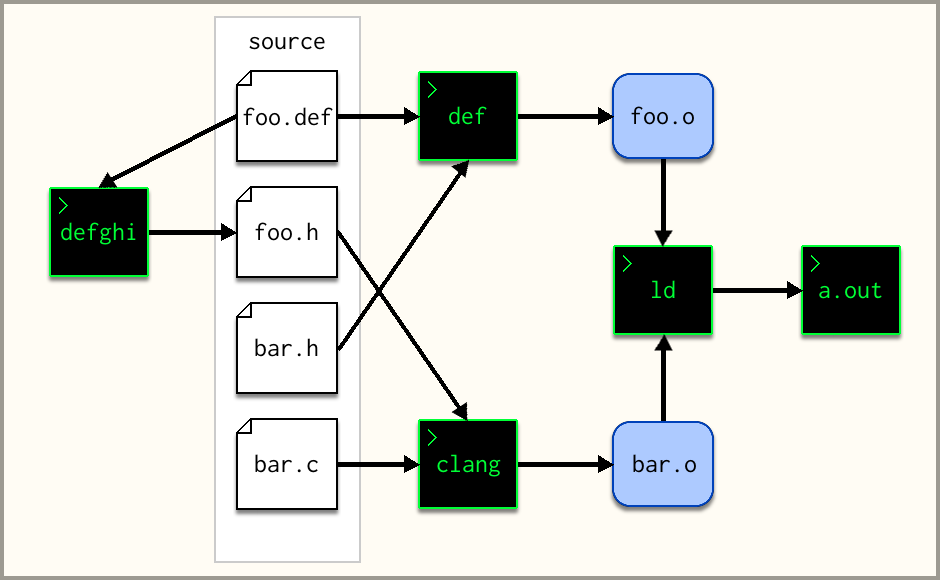
\includegraphics[scale=0.25]{gfx/seemless-integration}
        \caption{Integration between DEF and C source code can be done seemlessly by generating a C header file from the DEF source file, using the \texttt{defghi} utility, and importing/including the necessary header files into the respective source files.  Objects can be linked together as usual.}
        \label{fig:seemless-integration}
\end{figure}

DEF provides primitives for traditional low-level memory management in the form of \texttt{new} and \texttt{delete}, but also adds a \texttt{retire} keyword for use with pointers that may be visible to multiple threads.  The expectation is that memory can be allocated and deallocated, just as it is in normal C programs, and \texttt{new} and \texttt{delete} can be configured to use an application-specific allocator, since performance programmers generally look for one that performs best on their application.  But when memory is shared in a concurrent data structure, \textit{invisible readers}, threads that perform nothing but read operations on a node (and are, therefore, invisible to a thread that might want to free it), memory can be retired and tracked by a special-purpose runtime.

The rationale is that no tracking needs to take place on most memory in an application, and that the programmer has a good sense of when memory can \textit{probably} be deallocated (e.g., when a node is removed from the structure).  \texttt{retire} is a hint the programmer provides to the application.  As opposed to a garbage collector, that tracks and traces all memory it allocates, \texttt{retire} allows DEF to provide a more streamlined approach.

Design-wise, DEF's goal is to be good at the things C is good at, but also provide support for development of concurrent data structures.  The criteria are summarized, briefly:

\begin{enumerate}
        \item Achieve high performance on a single core, competitive with C.
        \item Facilitate development of modular concurrent data structures that expose only their interfaces to callers.
        \item Work as a drop-in replacement for C when interoperating with other programming languages.
\end{enumerate}

By default, DEF's native runtimes are the C runtime library and those that are required for support for concurrency (Forkscan\cite{Forkscan}) and parallelism (Cilk\cite{BlumofeCilk}).  Adding DEF to an existing application, therefore, creates no additional burden or potential dependency conflicts.

As proof of concept, we implemented a benchmark suite including various concurrent data structures in DEF with corresponding implementations in C.  Since C benchmarks often forgo memory reclamation altogether, or reuse memory based on knowledge of the benchmark usage patterns,\cite{Synchrobench}\cite{Scal} the C implementations in our benchmark are leaky.  (brief mention of results)


\section{Related Work}

The three core components of this work are the language design around memory reclamation, integration with C code bases, and the selection of concurrent data structures implemented in the benchmark.  Other design elements of the language are beyond the scope of this paper, and language features are introduced, briefly, as required in the Implementation section.

\subsection{Memory Reclamation}

In the context of concurrent data structures, modularity is defined primarily by memory management.  The API of a library is not identical to how much of its implementation it exposes.  Restrictions on where pointers can be stored or how long the caller is allowed to hold onto them are part of the profile of a library.  A modular language doesn't impose those kinds of requirements on users of libraries written in that language.

\paragraph{Unmanaged Languages} Numerous schemes have been devised for memory management of concurrent data structures in unmanaged languages.  In general, they are not automatic -- they place constraints on the programmer as to where pointers may be stored or when and how they may be dereferenced.  Nevertheless, they are successfully employed in real world applications, and are worth discussing.

\textit{Reference counting} can be applied to certain kinds of concurrent data structures\cite{DMMS, GPST09}.  Whenever a thread is ``looking at'' a shared object, it increments the object's reference counter, and decrements it again when it's done.  When the counter reaches zero, the object can be reclaimed.  This could, in principle, be automated within an unmanaged language, but it's costly to add a write on each object that's viewed, especially for structures where the most common operations are reads.  Reference counting also doesn't apply to data structures that have cycles, since removing a node with a child that references it will never be reclaimed.  And, as mentioned above, a caller into a library that uses it must know about it.

\textit{Pointer-based} mechanisms, such as Hazard Pointers\cite{HP, DTA, PassTheBuck}, typically impose lower performance penalties.  Instead of contending on shared memory, threads write to private memory, recording the objects they see.  Their private records are only viewed by other threads that actually want to free objects, so contention is lower.  There is still a write for every read, however, and they introduce memory fences to ensure their changes are visible other threads, introducing overhead per operation.  Efforts have been made to avoid the use of the costly memory barrier.\cite{MauriceCadence}  Additionally, a thread that wants to drop a reference must know that it's protected by a hazard pointer and remove it from its list, making something of the structure's implementation visible to users.

\textit{Quiescence-based} techniques\cite{FraserH07, Harris, Hart} are often performance competitive with implementations that leak memory.  These define \textit{epochs} in which references may be freely held and dropped arbitrarily.  Epochs have well-defined bounds, allowing the system to ``prove'' that there cannot be any outstanding references to nodes waiting for deletion, eliminating overhead per operation.  However, callers define epoch boundaries and prohibit the transfer of pointers across those boundaries; an exposed implementation.

In each of these cases, a concurrency library written with the given technique necessarily requires users of that library to know something about how memory is tracked, and what contracts must be honored to ensure memory isn't leaked and that invalidated memory isn't dereferenced.  That's acceptable in many applications, but it isn't modular.

\paragraph{Managed Languages} The other extreme is garbage collection.  In one respect, a garbage collector is ideal because callers can do as they please with references with the caveat that the conservative collectors of low-level languages prohibit ``hiding'' pointers with, e.g., XOR.  A caller into a library need not understand how the data structure works, or even whether it is serial or concurrent.  For this reason, most modern languages use garbage collectors.  Even systems languages are increasingly applying GC.  The benefits are clear -- by design, GC imposes no overhead on individual operations, conservative collectors need not even have special type information from stack frames, and modern GC is fast with low wait times.\cite{ShahriyarBM14}

However, even among systems languages intended for high performance code, the garbage collectors have their own allocators that are non-trivial to swap out.\cite{Go, DotNetGC, D}  This is a design decision: Use GC or don't.  All heap memory or none is tracked by the garbage collector, even for objects that will never be transferred between threads.  The D programming language allows some configuration including the manual deallocation of memory allocated from the collector, but all objects are still tracked from the moment of allocation.\cite{DPhobos}

Being rigid about the choice of allocator is problematic for high performance programming.  For a fixed allocator, for example, Go can advertise that they achieve comparable performance to C on some code.  But C programmers can choose from many allocators suited to different kinds of workloads, and performance can differ radically based on that choice, particularly in a multithreaded environment.\cite{Hoard, TCMalloc, JEMalloc, Supermalloc}

This relates to modularity in that a language that has its own collector, or simply a C/C++ program with a preferred allocator, can conflict with a library written in a language with a different collector in unexpected ways.  GC for DEF could never be highly integrated with the language, or it would make working with another language's collector cumbersome.

DEF's requirements differ from those of managed languages in that the assumption is that the programmer handles the memory management of an object until told otherwise via \texttt{retire}.  This usage model means that the performance of a DEF application resembles that of an unmanaged language except insofar as nodes in concurrent data structures are being retired, or are dependent upon the other language's allocator (just as C would be in the same circumstances).

There's an additional performance benefit in this interface over GC, even for the concurrent data structures, themselves.  In a concurrent data structure, retiring objects as they are removed means that they \textit{probably} can be reclaimed and reallocated, because it's unlikely that other threads are holding references to more than a few of them.  Unlike GC, few objects are being tracked, and most tracked objects aren't live.

\paragraph{Rust} The Rust programming language has its own method of safely collecting memory in a multithreaded environment without GC: all memory is ``owned'' by a single function at any given time, and the compiler can statically prove when memory can be released.\cite{Rust}  When a function is called, not only is a pointer to an object passed, but also its ownership.  If the calling function wants to use the object again, the called child must explicitly relinquish ownership when it returns.  This imposes no run time overhead, but is merely information for the compiler to use to determine when an object becomes ownerless and can be deallocated.

Though correct and fast, this limits the applicability of Rust's model in its application to concurrent data structures, themselves.  The ``interesting stuff'' (for our purposes) is precisely where many threads may be operating on a single memory location at the same time.  Such a data structure could be written in another language and imported, or the safety features in Rust could be disabled in the module, but in either case, a different means of reclaiming memory is required.  That said, a Rust-written concurrency library used within a Rust application, really is modular.  Enough information, through the type, is provided to a caller that reference counting, or whatever other means, won't fail to be honored.  This is not true when integrating the library into a non-Rust application, however.

\paragraph{Automatic On-Demand} Automatic tracking need not be all-or-nothing.  StackTrack\cite{StackTrack}, ThreadScan\cite{Threadscan}, and Forkscan\cite{Forkscan} are automated memory reclamation systems based on periodic searches for references, but they only apply to memory explicitly designated for tracking.  ThreadScan and Forkscan impose no overhead on individual operations on data structures, which is particularly beneficial for obtaining maximal performance in read operations.  ThreadScan operates by periodically pausing all threads and making them search their own stacks for references.  No thread may return to work until all stacks have been searched, imposing a delay (albeit, limited in practice) until the slowest thread completes.  Additionally, no references can be permitted to escape user stacks.

Forkscan forks the process and searches for references in the resulting snapshot.  This imposes a delay on user threads while the fork takes place, but the delay isn't dependent upon the speed of any threads.  The search in the snapshot is also a complete scan of memory, so unless references are hidden (by XOR'ing or some other means), none will escape.  Like conservative GC, using a concurrency library that has Forkscan means that a caller can hold onto a reference for any amount of time and store it anywhere in memory.

For this reason, DEF uses Forkscan to satisfy the \texttt{retire} interface.  Users of libraries need not know how memory is tracked, merely that it won't leak.  Furthermore, Forkscan acts as an intermediate, transparent layer between an application and its allocator, so it permits a programmer to select the allocator that best fits the application.


\subsection{C Integration}

The benefits of C integration are numerous: The major computer operating systems are written in C,\cite{Linux, Darwin, WindowsKernel} the C runtime is ubiquitous and generally doesn't conflict with other language runtimes, and C is conducive to high performance programming.

Language designers and maintainers commonly provide support and documentation for how to integrate C modules into projects based in their languages.  Of the top ten most popular languages by pull request on Github,\cite{Octoverse} nine have native support for calling C code\cite{JavascriptCiface, PythonCiface, JavaCiface, RubyCiface, PHPCiface, DotNetCiface, GoCiface, CPPCIface} (the sole exception is CSS; C, in tenth place, obviously links with itself).

\begin{figure}[htbp!]
        \centering
        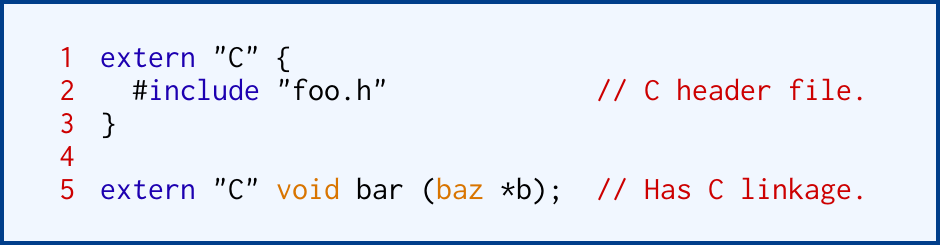
\includegraphics[scale=0.25]{gfx/extern}
        \caption{Example of C++ code that imports a header file from C and exports a function that can be used by a C module.}
        \label{fig:extern-example}
\end{figure}

Fig.~\ref{fig:extern-example} demonstrates that C++ goes to lengths to be compatible with C in both directions.  By using \texttt{extern \textquotedbl{}C\textquotedbl{}}, a symbol can be declared with C linkage, and since all of the native C types correspond to native types in C++, calling back-and-forth between languages is easy.  It means that C++ is compatible with any language with C hooks.  This is the only language we are aware of that has this degree of integration.

Both directions are integral to the design of DEF.  Even though many elements of DEF's syntax are inspired by C, it isn't interchangeable even in simple cases, as C++ is.  Nevertheless, \textit{well-behaved} C header files can be imported directly into DEF.  A header is well-behaved if, as included in a C source file, it satisfies the C parser in itself -- neither expecting tokens prior to beginning, nor requiring tokens after.  Because headers are typically written as interface files, most are well-behaved including all of the standard libraries.


\subsection{Concurrent Data Structures}


\section{Implementation}

For a thorough examination of the language, DEF has a language wiki,\cite{DEFWiki} however, a brief comparison with C is provided to show that it is, in fact, close to the machine in the same way that C is, albeit with a different syntax.  The DEF compiler is based on the Tapir branch of LLVM, that adds fork-join parallelism primitives.\cite{TAPIR,LLVM}  The front-end is principly written in OCaml, but includes some C++.

Likewise, the \texttt{defghi} utility is written in OCaml,\cite{DEF} and is described in the Compatibility section.

Finally, the suite of microbenchmarks was developed in DEF and C with the driver in DEF.  The concurrent set data structures selected for the suite were chosen for high performance and variety.

\subsection{Close to the Machine}

\begin{figure}[htbp!]
        \centering
        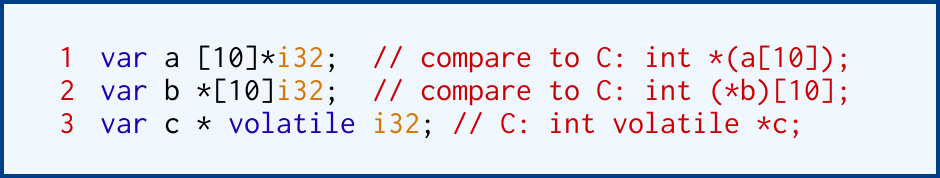
\includegraphics[scale=0.25]{gfx/types}
        \caption{Examples of variable declarations in DEF.  C allows the parentheses to be omitted in the first case, though they're provided to make precedence explicit.}
        \label{fig:types}
\end{figure}

Syntactically, DEF has some similarity to C with the most apparent difference being that scopes are denoted by keywords instead of curly braces (e.g., \texttt{if}/\texttt{then} and \texttt{fi}, \texttt{do} and \texttt{od}, etc.) allowing curly braces to be repurposed for tuples.  Native types specify a bit width, so C's \texttt{int} on most systems corresponds to DEF's \texttt{i32}.  Types are also designed to read left-to-right, so the return type in a function declaration has been moved to the right using an arrow notation similar to ML-like languages or Go.  For more complicated types, fig.~\ref{fig:types} gives an example of left-to-rightness where no parentheses are needed to distinguish an array of pointers to integers (line 1) from a pointer to an array of integers (line 2).

The expressibility is equivalent to C.  Arrays, for example, contain no metadata and can appear on the stack or on the heap.  DEF is able to commit to native integers and floating point variables of specific width, however, because architectures have largely settled on them.  C acknowledges this as of the C99 standard with types like \texttt{int32\_t} defined in the \texttt{stdint.h} header file.(cite C99)

\begin{figure}[htbp!]
        \centering
        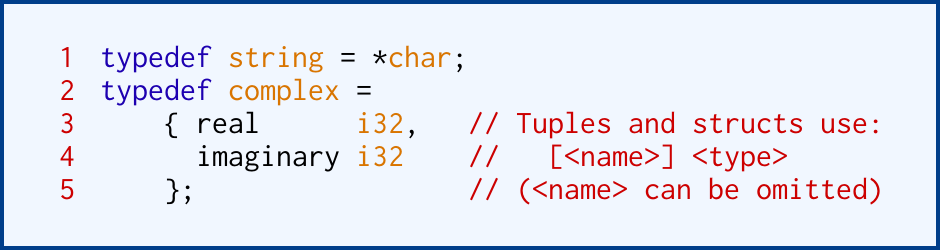
\includegraphics[scale=0.25]{gfx/typedef}
        \caption{Defining types with \texttt{typedef}.}
        \label{fig:typedef}
\end{figure}

Types are defined with the \texttt{typedef} keyword.  Figure \ref{fig:typedef} shows two examples: a C-style \texttt{string} type is defined on line 1, and a complex number struct is defined on lines 2-5.  The struct's actual definition is identical to tuple syntax, though tuples typically omit the member names.  Worthy of note is that tuples in DEF really are just anonymous structs, in keeping with the design goal of interchangeability with C.  Whereas in many languages tuples are allocated on the heap and garbage collected, in DEF they're allocated however a named struct would be in C.  Locating a struct or tuple on the heap requires explicit allocation.  Fig.~\ref{fig:window-find} provides a \texttt{window\_{}find} function declaration from the Harris lock-free linked list\cite{Harris} in Herlihy and Shavit,\cite{HSBook} as expressed in C (lines 2-6) and DEF (lines 9-10).  In both cases, the struct is returned by value on the stack.  A pointer, in both languages, would require explicit pointer syntax.

\begin{figure}[htbp!]
        \centering
        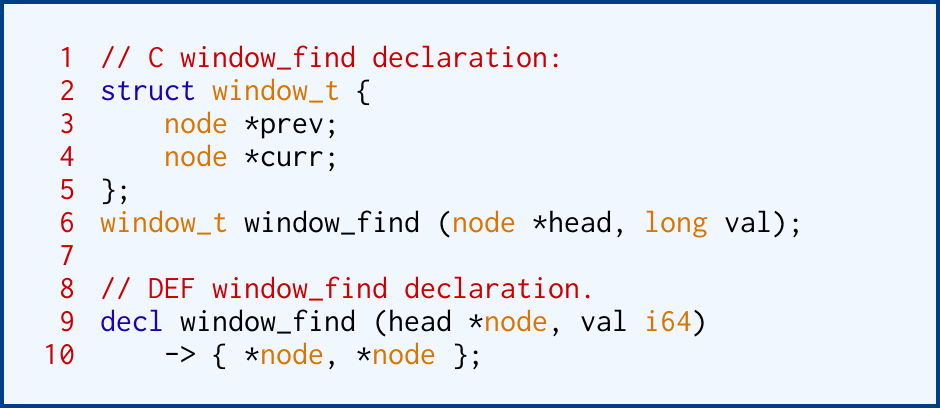
\includegraphics[scale=0.25]{gfx/window-find}
        \caption{Equivalent \texttt{window\_{}find} declarations in C and DEF.  The DEF tuple is an unnamed equivalent of C's \texttt{window\_{}t}.}
        \label{fig:window-find}
\end{figure}

Binary Read-Modify-Write (RMW) operations with sequential consistency can be expressed by applying an \texttt{atomic} modifier to the target operation.  Fig.~\ref{fig:atomic} shows an example of \texttt{atomic} being used to add into the variable \texttt{a}.

\begin{figure}[htbp!]
        \centering
        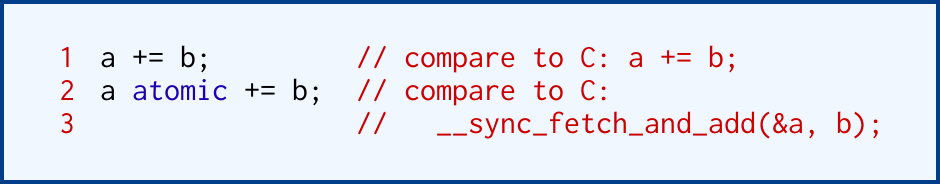
\includegraphics[scale=0.25]{gfx/atomic}
        \caption{Example of modifying a non-RMW operation to make it RMW in DEF.  The C atomic is available since C11.}
        \label{fig:atomic}
\end{figure}

Despite the difference in syntax, DEF exhibits the same kind of expressibility as C in data layout and instruction generation.  There aren't unexpected hidden costs in operations or types, allowing a programmer to tune DEF code for performance in the same way as one would do for C.

\subsection{Modularity}

As above, modularity is decided by the profile presented to users of a library.  In a concurrent data structure, what does a programmer need to know about pointers returned from thus-and-such a function call?  What are the restrictions?

DEF has no native allocator.  Allocating memory with \texttt{new} and deallocating it with \texttt{delete}, use \texttt{malloc} and \texttt{free}, respectively.  Since DEF's memory reclamation system is implemented using Forkscan, they implicitly use Forkscan's \texttt{malloc} and \texttt{free} wrappers, but the overhead of this indirection is undetectable in trials.  Independent of implementation, memory allocated with \texttt{new} is untracked.  Memory can be passed freely between DEF and C, and a pointer acquired in C through \texttt{malloc} can be deleted in DEF, and one acquired in DEF through \texttt{new} can be freed in C.

Moreover, \texttt{new} and \texttt{delete}, as applied to non-shared memory, are conveniences-only.  Mixing allocators or interfacing with a language with hooks to an external garbage collector is as trivial (or as complex) in DEF as it is in C because all memory is treated in exactly the same way.

The exception to this is in the use of \texttt{retire} to flag a pointer for tracking.  \texttt{retire} cannot be applied arbitrarily to pointers since there is no way to determine origin.  DEF assumes that a retired node was allocated with the same allocator used by \texttt{new}.  Implementation-wise, Forkscan requires knowledge of the \texttt{free} and \texttt{malloc\_{}usable\_{}size} corresponding to the \texttt{malloc} that was used to acquire the memory.  More broadly, it's hard to see how any implementation could call the correct \texttt{free} on a retired node unless it corresponded to the known \texttt{malloc} for the same reason.  This is not especially burdensome to programmers since mixing allocators is typically frowned upon.

A final restriction on \texttt{retire} is that it may only be called on a pointer, once.  If multiple threads retire the same memory, the behavior is undefined.  In practice, it acts like a double-free because the reclamation system may perform a double-free.  A good usage model is the thread that successfully removes a node from the concurrent data structure is the one that should retire it.  This makes its use intuitive because code looks like the familiar serial model where \texttt{retire} is replaced by \texttt{delete}.

Forkscan was modified to accommodate these semantics.  When Forkscan completes a memory sweep, it creates a pool of pointers known to have no outstanding references in the user program.  As designed, every call to \texttt{forkscan\_{}malloc} first frees a few of these pointers.  But this creates a dependency on \texttt{forkscan\_{}malloc}.  If a C module naively, repeatedly calls \texttt{malloc} (as opposed to \texttt{forkscan\_{}malloc}), even from the correct allocator, and gives the memory to a DEF module that retires it, unless the DEF module is also independently allocating its own memory with \texttt{new}, none of the retired memory will ever be reused.  This is a practical leak.  The modification moved the burden from \texttt{forkscan\_{}malloc} to \texttt{forkscan\_retire}, eliminating the dependency.

This produced no discernable difference in performance.  The reasoning for the original design was that freeing memory and then immediately allocating would likely return a pointer to memory that was already in the cache.  High performance allocators tend to have this property.  Changing the location of the burden didn't affect performance because, even if \texttt{malloc} wasn't called immediately after \texttt{free}, the delay between retiring and allocating memory wasn't very great, and the allocated memory was probably still in the cache.  Since some of the concurrent data structures tested were among the most high-performance known, we reason that the change has little or no effect on performance.  Even in a producer/consumer application, where \texttt{malloc} is being called with high frequency such that whether memory in cache has a measurable impact on performance, the likelihood is that the producer is getting memory from the cache in a high performance allocator, anyway.

\subsection{Compatibility}

C++ is the gold-standard for interfacing with C.  As mentioned above, C header files can be included directly into C++ files, and C++ functions can be declared with C linkage.  Features like templates, classes, and member functions of structs, can't be exported to C, but anything C-like can be.  Given DEF's syntactic differences, even for features it holds in common with C, sharing DEF interface (\texttt{.defi}) files directly with C is impractical.  However, most of the function-level features have a one-to-one correspondence with C.  Therefore, the compiler is accompanied by a utility, \texttt{defghi}, for generating headers and interface files from DEF source files.

Generating headers and interface files is assisted by a formal approach to module interfaces.  A subtle distinction from C is that DEF types, functions, and globally-scoped variables are local to the module in which they appear, by default.  C's default is external visibility, and local symbols must be marked \texttt{static} by the programmer.  In contrast, DEF requires programmers to mark symbols with \texttt{export} in order to make them visible.

Since the differences are syntactic, generating header files from \texttt{defghi} is simple.  Any type, global variable, or function marked \texttt{export} has its declation unparsed into C and pretty-printed into the header.

The other direction, importing C definitions into DEF, involves recognizing headers by filename extension and passing them through a C parser.  Clang, the LLVM C compiler, collects all type definitions and function and global variable declarations, and DEF converts them into its own internal representation.  Therefore, DEF can import C headers directly as if they were native DEF.

There are two limitations to this: DEF can't import actual C functions (as opposed to function declarations), and C macros aren't resolved except where they appear in a header file itself.  In the first case, functions in header files are a planned feature that was deprioritized since they're uncommon in the C standard library, and it was reasoned that high performance programmers often do intermodule optimization, negating the value of putting them in headers.  In the second case, DEF does not yet have macros of its own, and a naive implementation of incorporating C macros might conflict with a well-designed DEF macro language.  Since C macros are simple text-substitution, integration into a language with a different syntax is another problem, altogether.

Even with the current limitations, however, DEF is able to import the C standard libraries, use their types, call their functions, and access their global variables.

\subsection{Concurrent Data Structures}


The are two classes of data-structures chosen for our comparison, sets and priority queues each with their own benchmark driver. In the set benchmark, items are randomly added and removed at a specified update rate. For the priority queues either a random element is added or the minimum element is removed.

\paragraph{Skip List} A fixed-height lock-free skip list was included as a well-known probabilistic concurrent data structure.  Each node contains one value, and the nodes are arranged in a list with a set of one or more forward pointers.  Each forward pointer points to the next node with at least that height, and the height of all nodes averages two.  Operations take logarithmic time, as they would in a binary tree, but tend to have better cache behavior. A node is retired by the thread that swings the lowest height pointer during the removal of a node; a one-line change to the algorithm as described in Herlihy-Shavit.\cite{HSBook}

\paragraph{Hash Table} The lock-free separate chaining hash table performed favorably in Michael's tests.\cite{HashTables} Each bucket in the hash table contains a lock-free linked list by Harris.\cite{Harris} The list at each bucket is sorted and allows for early search termination. Like the Harris list a window of nodes is kept during the \texttt{find} procedure and used in insertion and removal. Nodes in the list are removed by marking the current node's next pointer, effectively locking that node. This stops another node from being inserted in front of the current node marked for deletion. Finally the removing thread swings the previous node's next pointer to the next pointer of the current node being removed, splicing the current node out of the list. Other threads that see a marked next pointer help remove the marked node from the list, making the remove operations cooperative and lock-free. During out experiments the average list length at each bucket was kept at 36 nodes.

\paragraph{Binary Tree} The fast concurrent lock-free binary search tree by Natarajan and Mittal is a recent concurrent data structure that operates by marking edges rather than nodes.\cite{LFBinaryTree} The algorithm is relative simple and fast due to the lack of any rebalancing algorithm. Rebalancing algorithms are a source of contention as some require a potentially global data-structure reorganisation. The data-structure is an external binary tree, meaning the values of the set are stored in the leaf nodes rather than throughout the tree. The internal nodes are only for routing and serve no other purpose. The work-horse of the data-structure is the \texttt{seek} method. Like the Harris linked list, \texttt{seek} constructs a window of the tree while searching. \texttt{Seek} will exclude nodes that have been marked for deletion as those nodes cannot be valid ancestors for replacement when removing. The tree contains a fixed amount of nodes which are never removed so that there will always be a valid node family tree. Removing a node is a two stage process and requires two bits. The two bits represent \textit{flagging} and \textit{tagging} of an edge. To remove a node first the thread first marks the parent's edge to the node, this mark is a flagging operation. The second marking takes place in the \texttt{cleanup} method, \texttt{cleanup} is run when a modifying operation sees a \textit{flagged} edge to a node. The second marking is done on the sibling node of the node to be removed, this marking is called \textit{tagging}. Once both edges (of the parent) have been marked no other modifying operation can occur and now the parent and the node to be removed can be unlinked. Like deletion, retiring is a two stage process. The thread that initially injects the deletion, via \textit{flagging} an edge, retires the leaf node. Later the thread that replaces the successor in \texttt{cleanup} with the sibling of the to be deleted node retires the successor node.

% \paragraph{Shavit Lotan Queue} This was included as an example of a skip list-based priority queue. \cite{ShavitLotanQueue} The Shavit Lotan Queue is a lock-free priority queue data-structure where the \texttt{pop-min} method traverses the lowest height/level of the skip list. Since the skip list is a series of sorted linked lists, with the lowest height/level containing all values, threads can remove the top items from the list which have the highest priority. Deletion is done logically, using the atomic swap (or similar CAS) to mark a node as deleted and then physically removing that node at that point or sometime after. Timestamps can be added to each node in order to make the list linearisable \cite{Linearizability}, otherwise the structure is quiescently consistent (cite). As in the skip list, the node is retired by the thread that swings its lowest height pointer.

\paragraph{Lind{\'e}n Jonsson Queue} This was included as an example of a skip list-based priority queue. \cite{LindenPriority} The Lind{\'e}n Jonsson Queue is a lock-free priority queue data-structure where the \texttt{pop-min} method traverses the lowest height/level of the skip list. Since the skip list is a series of sorted linked lists, with the lowest height/level containing all values, threads can remove the top items from the list which have the highest priority. Deletion is done logically, using the atomic swap (or similar CAS) to mark a node as deleted with physical deletion delayed until some point after. Physical deletion is done in batches and is quite efficient, the size of the batch is specified ahead of time. The thread which performs physical deletion is responsible for retiring the nodes.

\paragraph{SprayList} Finally, the benchmark includes a SprayList priority queue.\cite{SprayList} The SprayList is based on a skip list, but the node to remove is selected probabilistically from near the beginning to reduce contention. This probabilistic walk is referred to as the \textit{spray} and is paramount to reducing contention from threads. The SprayList is a relaxed concurrent data-structure whereby \texttt{pop-min} will remove from a range of top items in the list. The range and other parameters of the \textit{spray} are initialised by the number of expected threads (concurrency) acting on the queue. Because nodes closer to the beginning are less likely to be \textit{landed-on} after the \textit{spray}, padding nodes are added to the beginning of the list. Once the SprayList \textit{sprays} it will continue in the same fashion as the Lind{\'e}n Jonsson Queue and traverse the lowest level of the list until a deleted node is found. Under high contention the SprayList can scale significantly better than traditional concurrent priority queues, but it can be very sensitive to the choice of spray parameters. As in the skip list, the node is retired by the thread that swings its lowest height pointer.



\section{Experimental Results}

\subsection{Test Configuration}

Our benchmark was tested on a 72-core (4 sockets with 18 cores each capable of running 2 hardware threads, totalling 144 hardware threads) Intel Xeon machine clocked at 2.50 GHz with 512 GB of RAM and 4 memory banks. The machine is running Ubuntu 14.04 with kernel version 3.13.0-141. The with DEF code was compiled with DEF version 0.18.0a and the C code was compiled with Clang 6.0, and all code was compiled with -03 level of optimization.

During the benchmark threads were pinned programmatically to individual cores initially avoiding HyperThreading and later exhausting all individual execution units on a single CPU with the use of HyperThreading, before migrating to another CPU socket. JEMalloc\cite{JEMalloc} was used in all tests, as it had been in the Forkscan paper.\cite{Forkscan} The \texttt{numactl} Linux program was used to control which memory bank allocation was allowed to take place. The memory banks closest to the running CPUs were selected as they became active.

The microbenchmark measures the number of operations carried out over a specified amount of time rather than the time taken to execute a specified number of iterations. The rationale for this is threads finish their iterations before other threads. The remaining threads complete their iterations with less contention in the system, skewing the overall benchmark. Our benchmark reports the number of operations per second. The primary comparison is between the leaky C and the Forkscan enabled DEF implementations. Each benchmark is run for a total of 20 seconds each, with each configuration being sampled 5 times. The average of the runs is plotted with error bars show the maximum variation in each run.

\subsection{Benchmark Results}

\begin{figure}[htbp!]
  \centering
  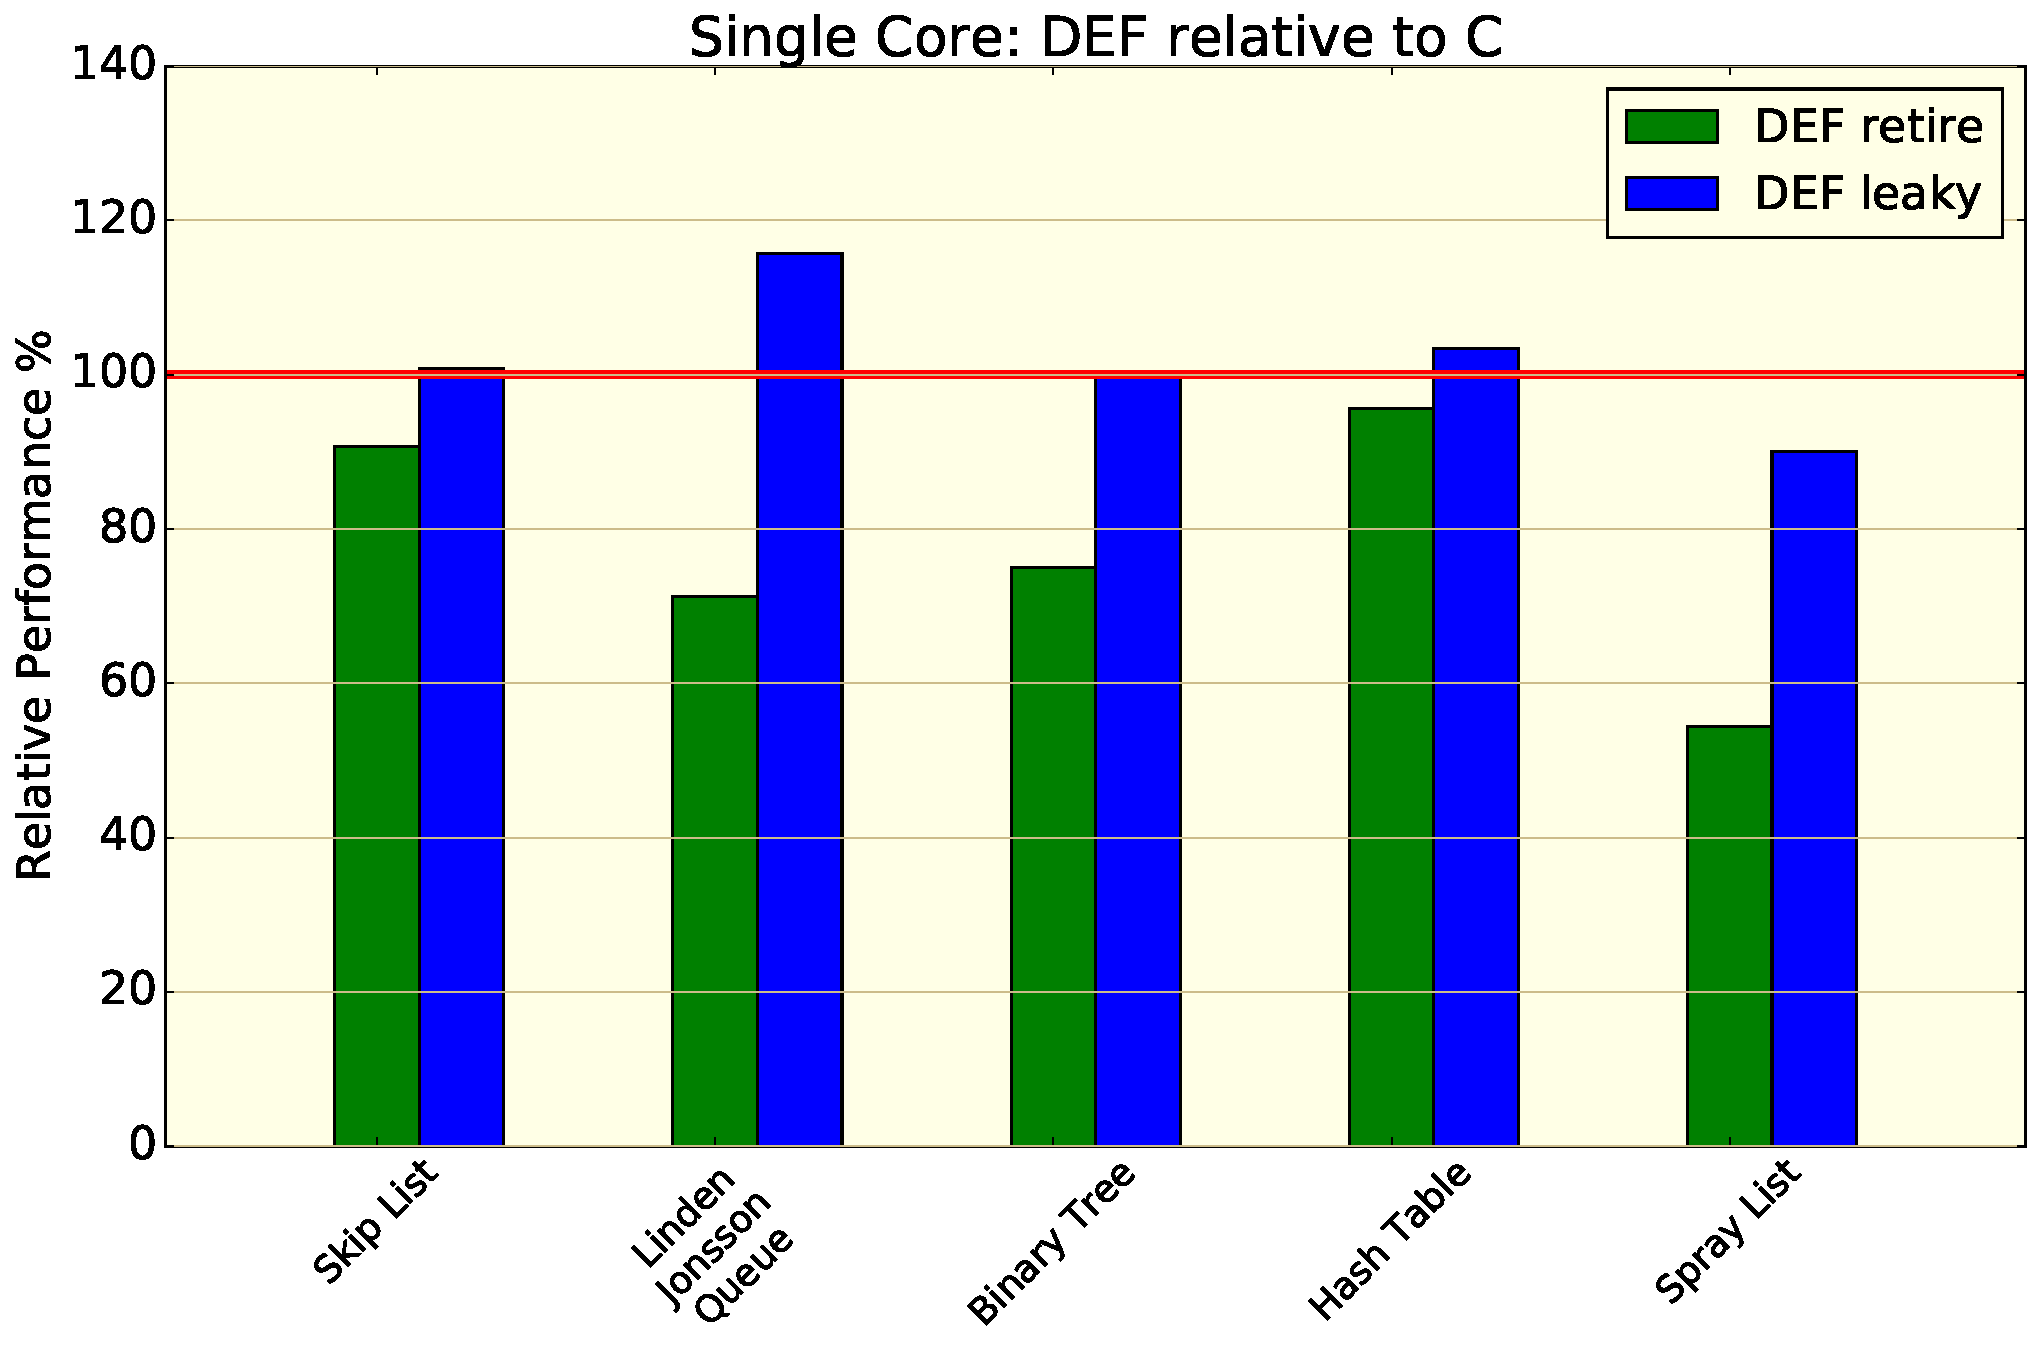
\includegraphics[scale=0.25]{gfx/RelativePerf.pdf}
  \caption{Relative performance of DEF to C on a single thread.  100\% is equivalent, and higher is better.}
  \label{fig:relativeperf}
\end{figure}

Figure \ref{fig:relativeperf} shows, for all benchmarks, single-threaded performance.  The set data structures are configured with 10\% updates, and the priority queue, naturally, are 100\% updates.  For an apples-to-apples comparison with C, a non-retiring version of the DEF code is presented.  This is a meaningful test because one expects a serial C data structure to perform better when \texttt{free} is never called than when it is, and it's no different for a concurrent data structure.  As designed, DEF is close to the machine and performs comparably in this case.  We attribute any performance distinctions to slight differences in code generation.

Minor degradation in performance is observed when memory is retired, except in the Lind\'en Jonsson Queue, which suffers from the burdened batch retires.

\begin{figure*}[tbp]
  \centering
  \raisebox{-0.5\height}{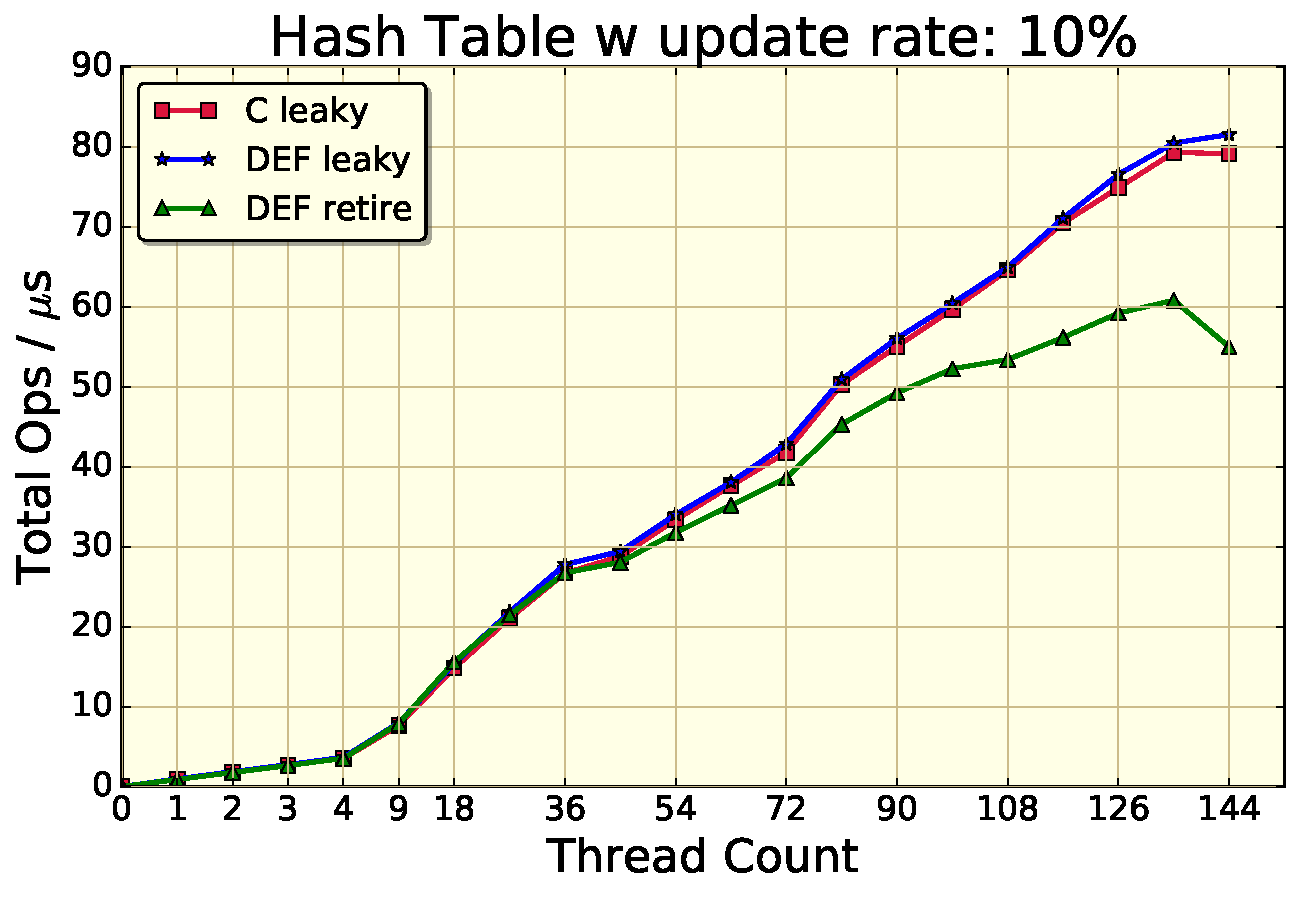
\includegraphics[scale=0.25]{gfx/HashTableLight.pdf}}
  \raisebox{-0.5\height}{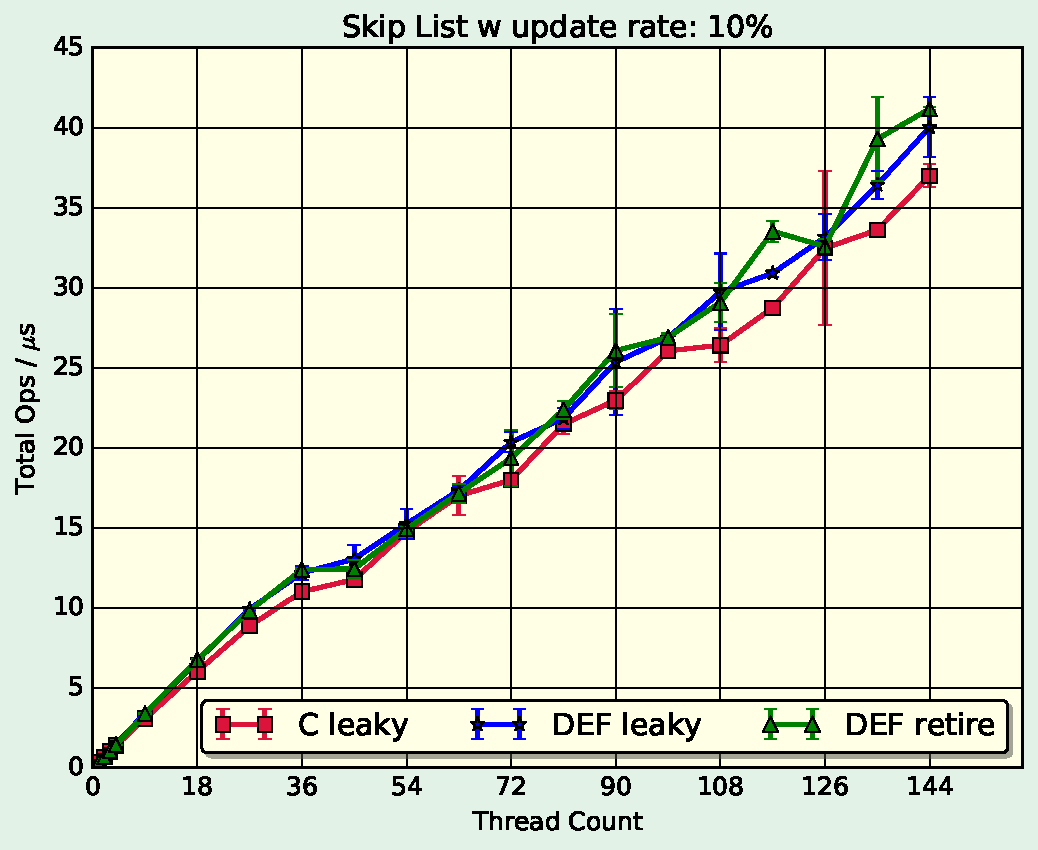
\includegraphics[scale=0.25]{gfx/SkipListLight.pdf}}
  \raisebox{-0.5\height}{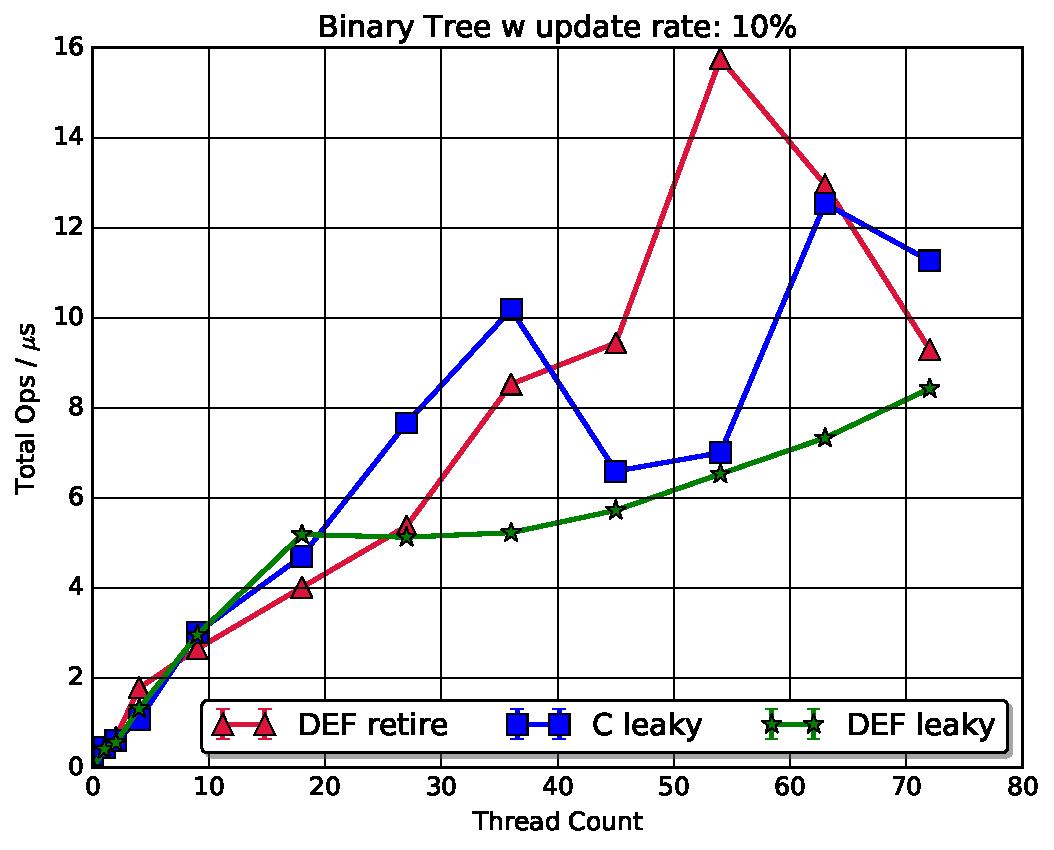
\includegraphics[scale=0.25]{gfx/BinaryTreeLight.pdf}}
  \raisebox{-0.5\height}{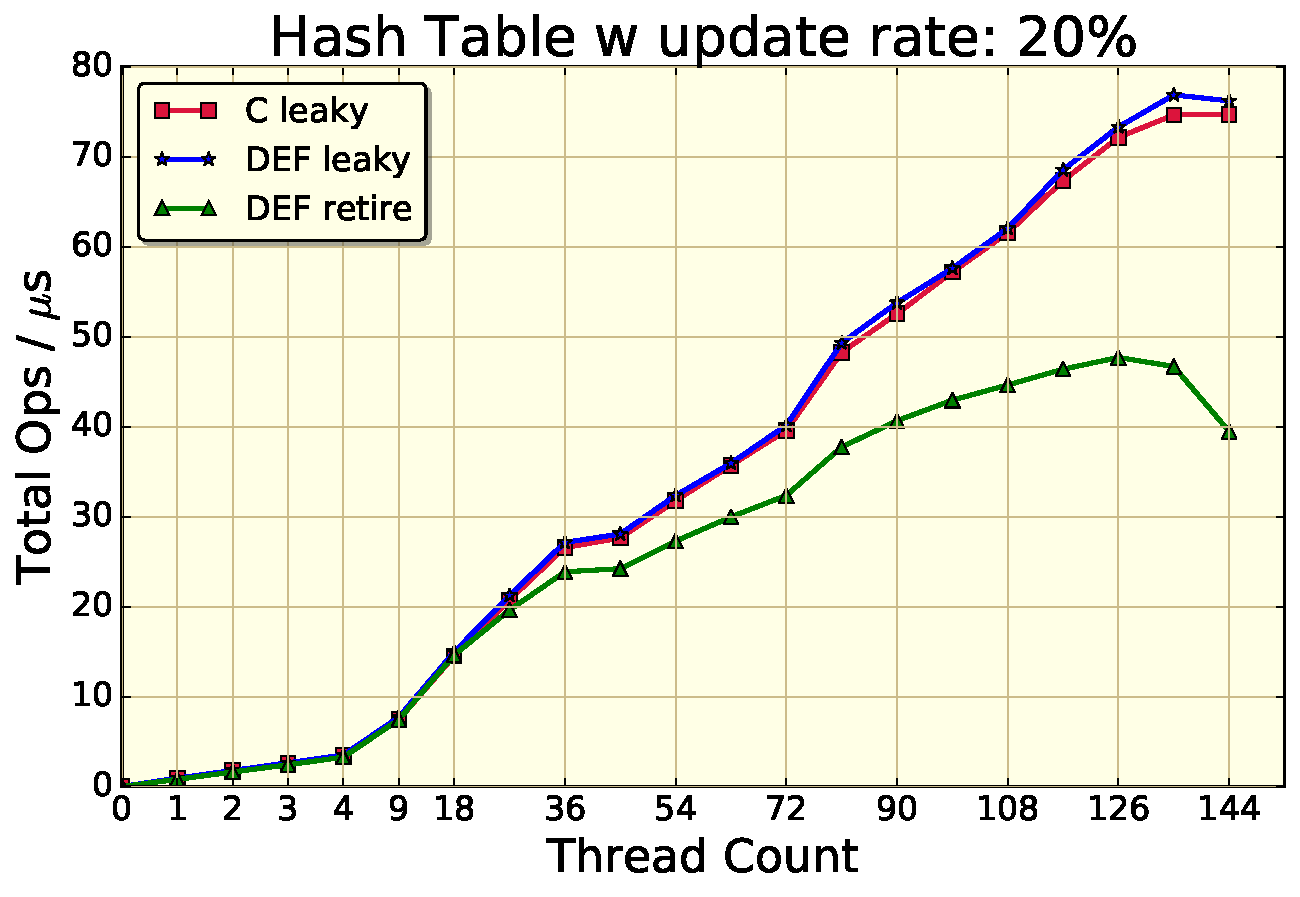
\includegraphics[scale=0.25]{gfx/HashTableMedium.pdf}}
  \raisebox{-0.5\height}{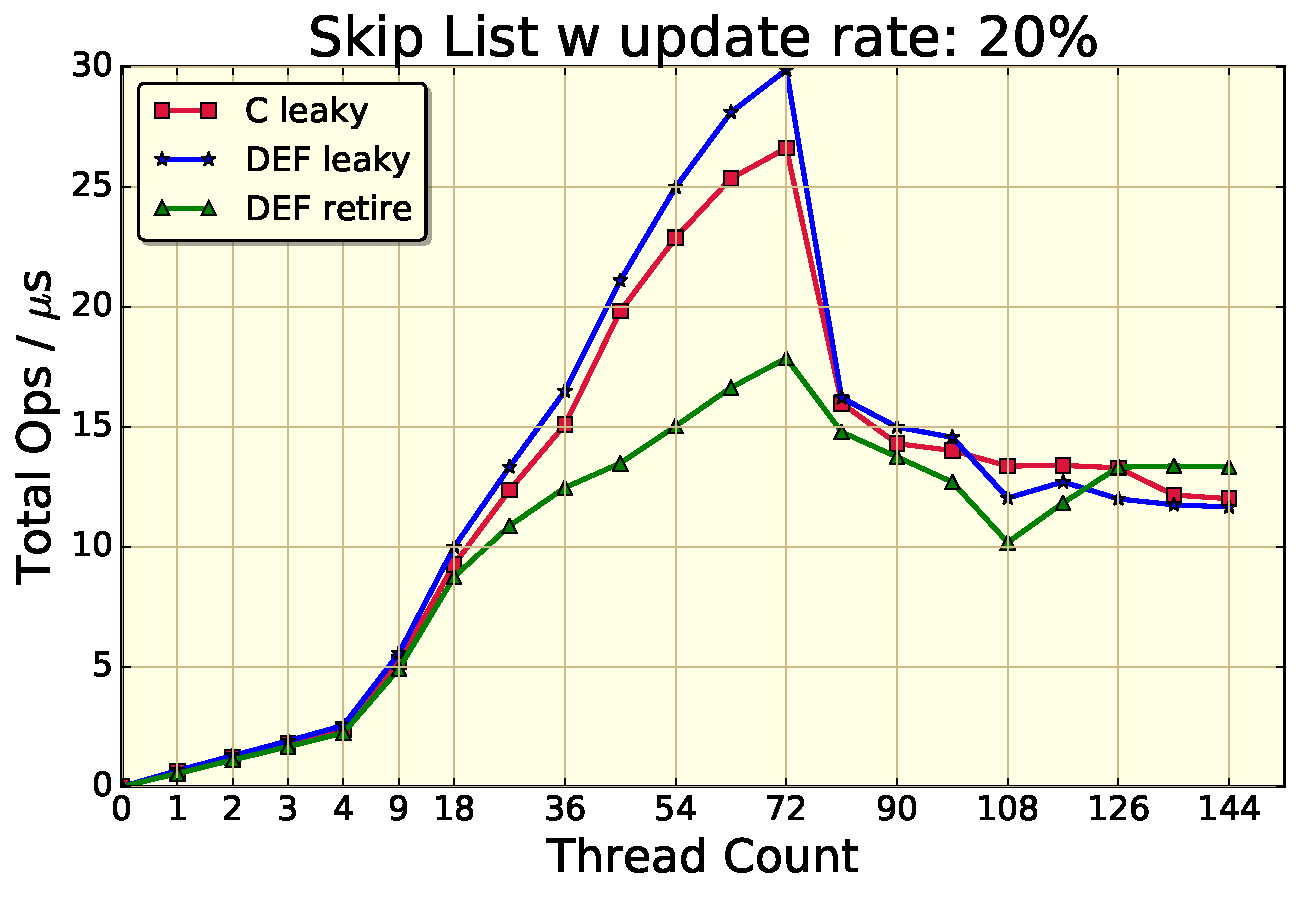
\includegraphics[scale=0.25]{gfx/SkipListMedium.pdf}}
  \raisebox{-0.5\height}{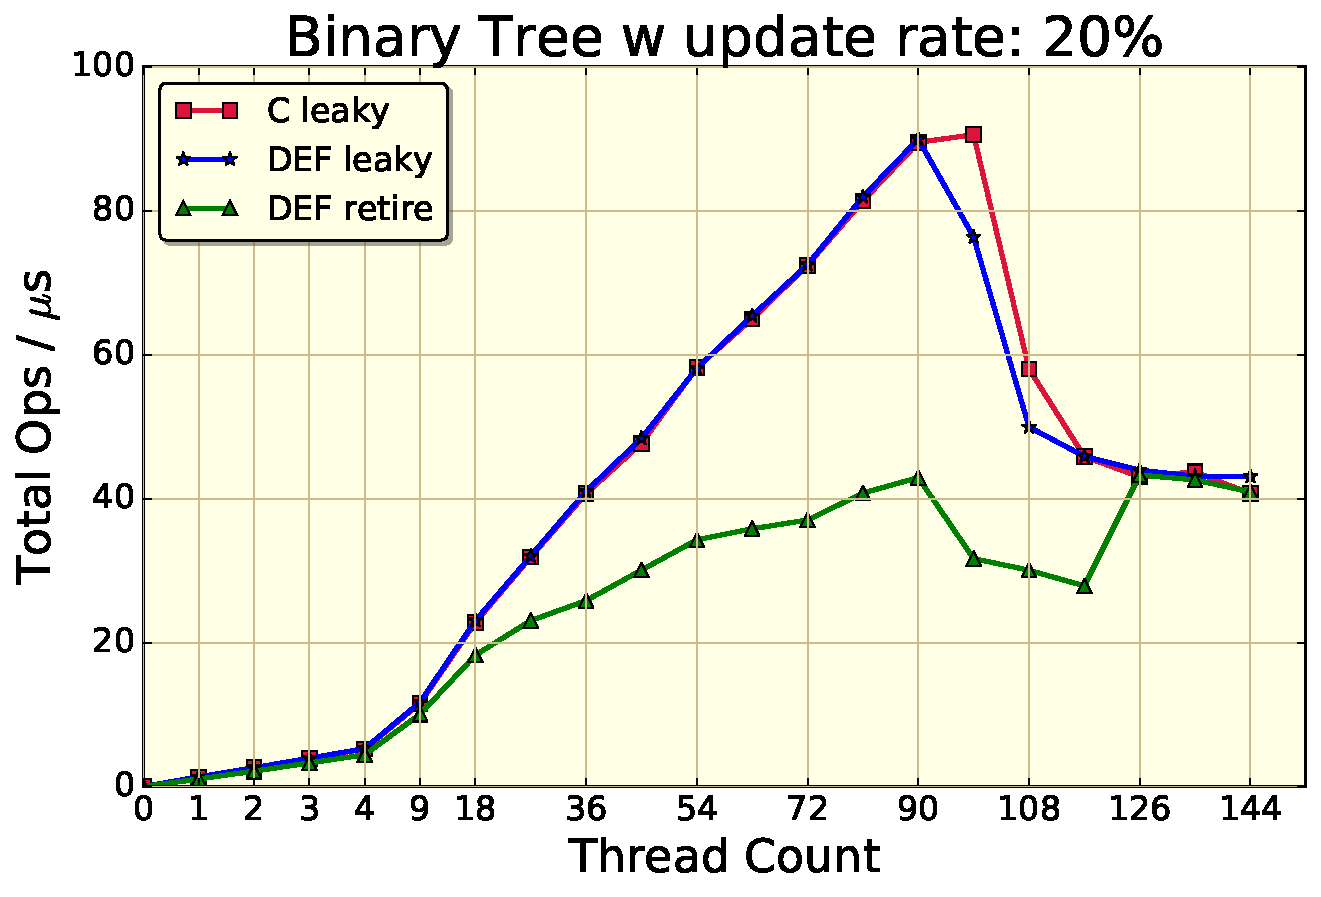
\includegraphics[scale=0.25]{gfx/BinaryTreeMedium.pdf}}
  \caption{Scalability graphs for the set data structures with 10\% (top row) and 20\% (bottom row) updates.}
  \label{fig:setdatastructures}
\end{figure*}

Scalability results for the set data structures with 10\% and 20\% updates are presented in figure \ref{fig:setdatastructures}.  20\% updates, on a set data structure, represents an extremely heavy workload.  10\% represents something more typical.  As above, the three configurations were tested: Leaky-DEF, DEF, and C (also leaky).

% Hashtable: node = 24
% Tree: node = 24
% Skip List: node = 172 (height 20)
% Shavit/Lotan: node = 180 (height 20)
% SprayList: node = 180 (height 20)

C and Leaky-DEF both scale similarly for all three structures.  The hash table scales linearly, performing only a few operations per microsecond worse on 144 threads at 20\% than at 10\%.  In the retiring version of the code, Forkscan is able to keep pace until the application saturates the first socket at 36 threads.  The decline at the high end is due to the fact that Forkscan creates a pool of child processes to perform its scan, up to 16, but since the application threads are pinned, the Forkscan threads get shifted around.

The skip list saturates the memory bandwidth with its enormous fixed-height nodes.  The peaks are merely shifted left in the 20\% executions versus 10\%, and don't rise as high (35 vs. 60 ops/$\mu$s).  Leaky DEF scales more quickly and, consequently, falls off sooner than the C version.  This is related to the aforementioned difference in code generation.  Nodes average two pointers instead of one, as in the hash table, making root finding slower when memory is reclaimed.  But its decline has the same cause as the leaky implementations: it hits the memory bandwidth at the same time.

The binary tree tests the limits of the memory reclamation implementation, which scales with the leaky versions, but has a more gradual slope.  At 10\% it declines at the end, just as the hash table did, and for the same reason.  The binary tree, exceeding the performance of this hash table (due to the list length of 36), involves more writing per update.  At 20\% updates, the leaky versions reach the memory bandwidth limits before they've run out of physical threads.

\begin{figure*}[tbp]
  \centering
  \raisebox{-0.5\height}{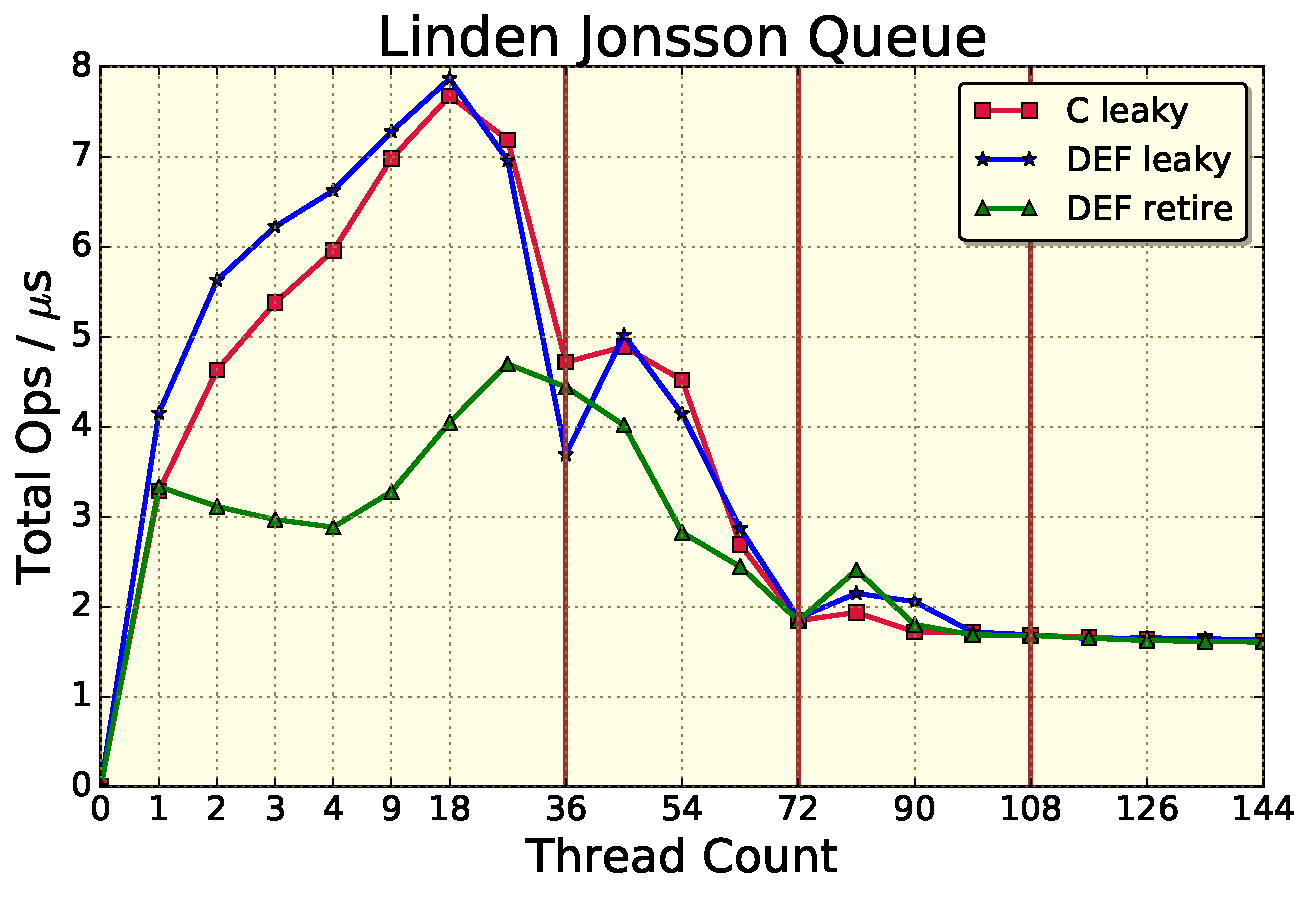
\includegraphics[scale=0.25]{gfx/LindenJonssonQueue.pdf}}
  \raisebox{-0.5\height}{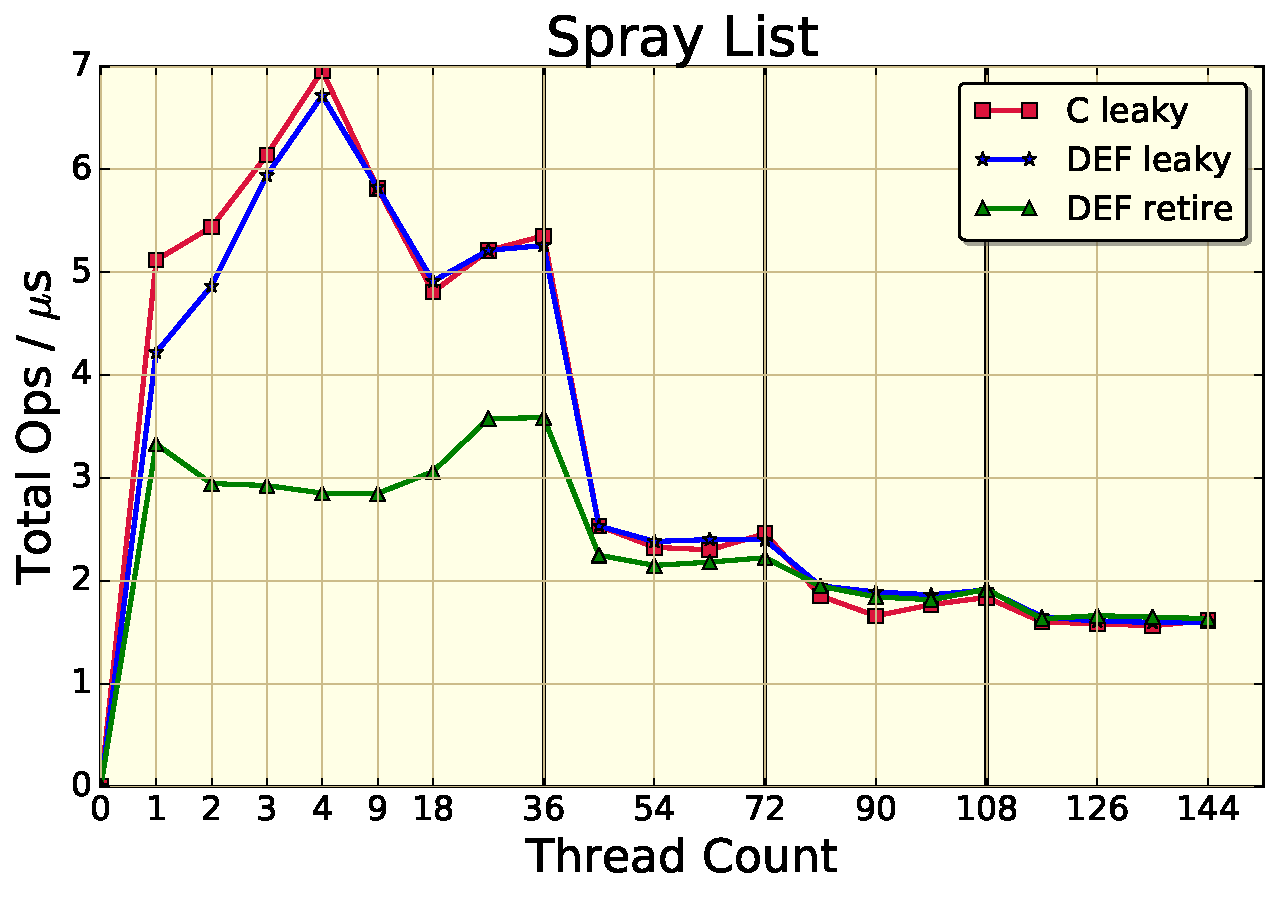
\includegraphics[scale=0.25]{gfx/SprayList.pdf}}
  \caption{Scalability graphs for the priority queues. The priority queues standard workload is 100\% updates.}
  \label{fig:priorityqueues}
\end{figure*}

Lastly, in figure \ref{fig:priorityqueues}, we tested the Lind{\'e}n Jonsson Queue and the SprayList priority queue.  The leaky implementations took a performance hit crossing the NUMA node boundary at 36 cores and never recovered.  One of the difficulties with a skip list-based priority queue is that many threads have a few early nodes in common in their caches.  As thread-counts increase, so do the number of invalidations, leading to the shape of the graph.  This is a worst-case data structure for Forkscan because priority queues are entirely updates, and the nodes are big (180 bytes, in this implementation).  However, again, the retiring DEF implementation has the same shape as the leaky ones.  It scales while they scale, and it's ultimately defeated by the same hurdle. The Lind{\'e}n Jonsson Queue beats the Spray List in our implementation. We found the Spray List's performance to be very sensitive to the parameter choice which scaled differently on for each thread count. One issue is that nodes were physically removed from the Spray List as soon as they were logically marked as deleted, increasing contention and degrading performance. 

In all of these structures, reclaiming memory scales up to the physical limits of the hardware, albeit with a gentler slope.  We attribute this to the on-demand aspect of memory tracking, versus at-allocation tracking; the memory that gets retired can mostly be de-allocated. Very little has to be recursively searched.



\section{Conclusion}

this is a conclusion.


%% Acknowledgments
\begin{acks}                            %% acks environment is optional
                                        %% contents suppressed with 'anonymous'
  %% Commands \grantsponsor{<sponsorID>}{<name>}{<url>} and
  %% \grantnum[<url>]{<sponsorID>}{<number>} should be used to
  %% acknowledge financial support and will be used by metadata
  %% extraction tools.
  This material is based upon work supported by the
  \grantsponsor{GS100000001}{National Science
    Foundation}{http://dx.doi.org/10.13039/100000001} under Grant
  No.~\grantnum{GS100000001}{nnnnnnn} and Grant
  No.~\grantnum{GS100000001}{mmmmmmm}.  Any opinions, findings, and
  conclusions or recommendations expressed in this material are those
  of the author and do not necessarily reflect the views of the
  National Science Foundation.
\end{acks}


%% Bibliography
\bibliography{bibliography}


%% Appendix
%\appendix
%\section{Appendix}

%Text of appendix \ldots

\end{document}
